\chapter{Estereoquímica}

\section{ATIVIDADE ÓTICA}

No começo do seculo XIX o físico francês Biot descobriu que inúmeras substâncias orgânicas naturais desviavam o plano da luz polarizada. Como a \textit{rotação ótica} ocorre mesmo quando os compostos estão na faze líquida, ela deve ser um fenômeno que ocorre em nível molecular. Alguns cristais, como o quartzo, também alteram o plano da luz polarizada, mas a rotação é, neste caso, um fenômeno devido ao cristal e não às moléculas, pois a rotação desaparece quando o cristal se funde ou é dissolvido. Tais casos, no entanto, não nos dizem respeito. '

Na última parte do seculo XIX, descobriu-se que existem pares de compostos que parecem ter estrutura e propriedades físicas idênticas, tais como ponto de fusão e solubilidade. Estes pares de compostos são diferenciados apenas pelo fato de, em solução, eles desviarem o plano da luz polarizada de um mesmo angulo, embora em sentidos opostos. Tais pares de compostos receberam, na época, o nome de \textit{isômeros óticos}. Antes de discutirmos as origens moleculares da atividade ótica, vamos descrever o polarímetro, o instrumento que permite o estudo da atividade ótica, assim como os princípios nos quais se baseia.

Um raio luminoso tem uma vibração eletromagnética associada a ele; esta vibração ocorre num plano perpendicular à linha de propagação do raio. Um feixe de luz comum consiste de um certo numero de raios, cada um com sua vibração electromagnética associada. As vibrações são sempre perpendiculares à linha de propagação, não sofrendo outras restrições. Portanto, as vibrações do feixe total ocorrem simultaneamente em todas as direções possíveis, como mostra a Figura \ref{figura_6_1}. Essas vibrações têm as propriedades de um vetor, de modo que uma vibração isolada pode ser considerada como resultante de duas componentes mutuamente perpendiculares. As vibrações do feixe podem, assim, ser consideradas como a soma de dois conjuntos separados de vibrações que são mutuamente perpendiculares.

\begin{figure}
    \centering
    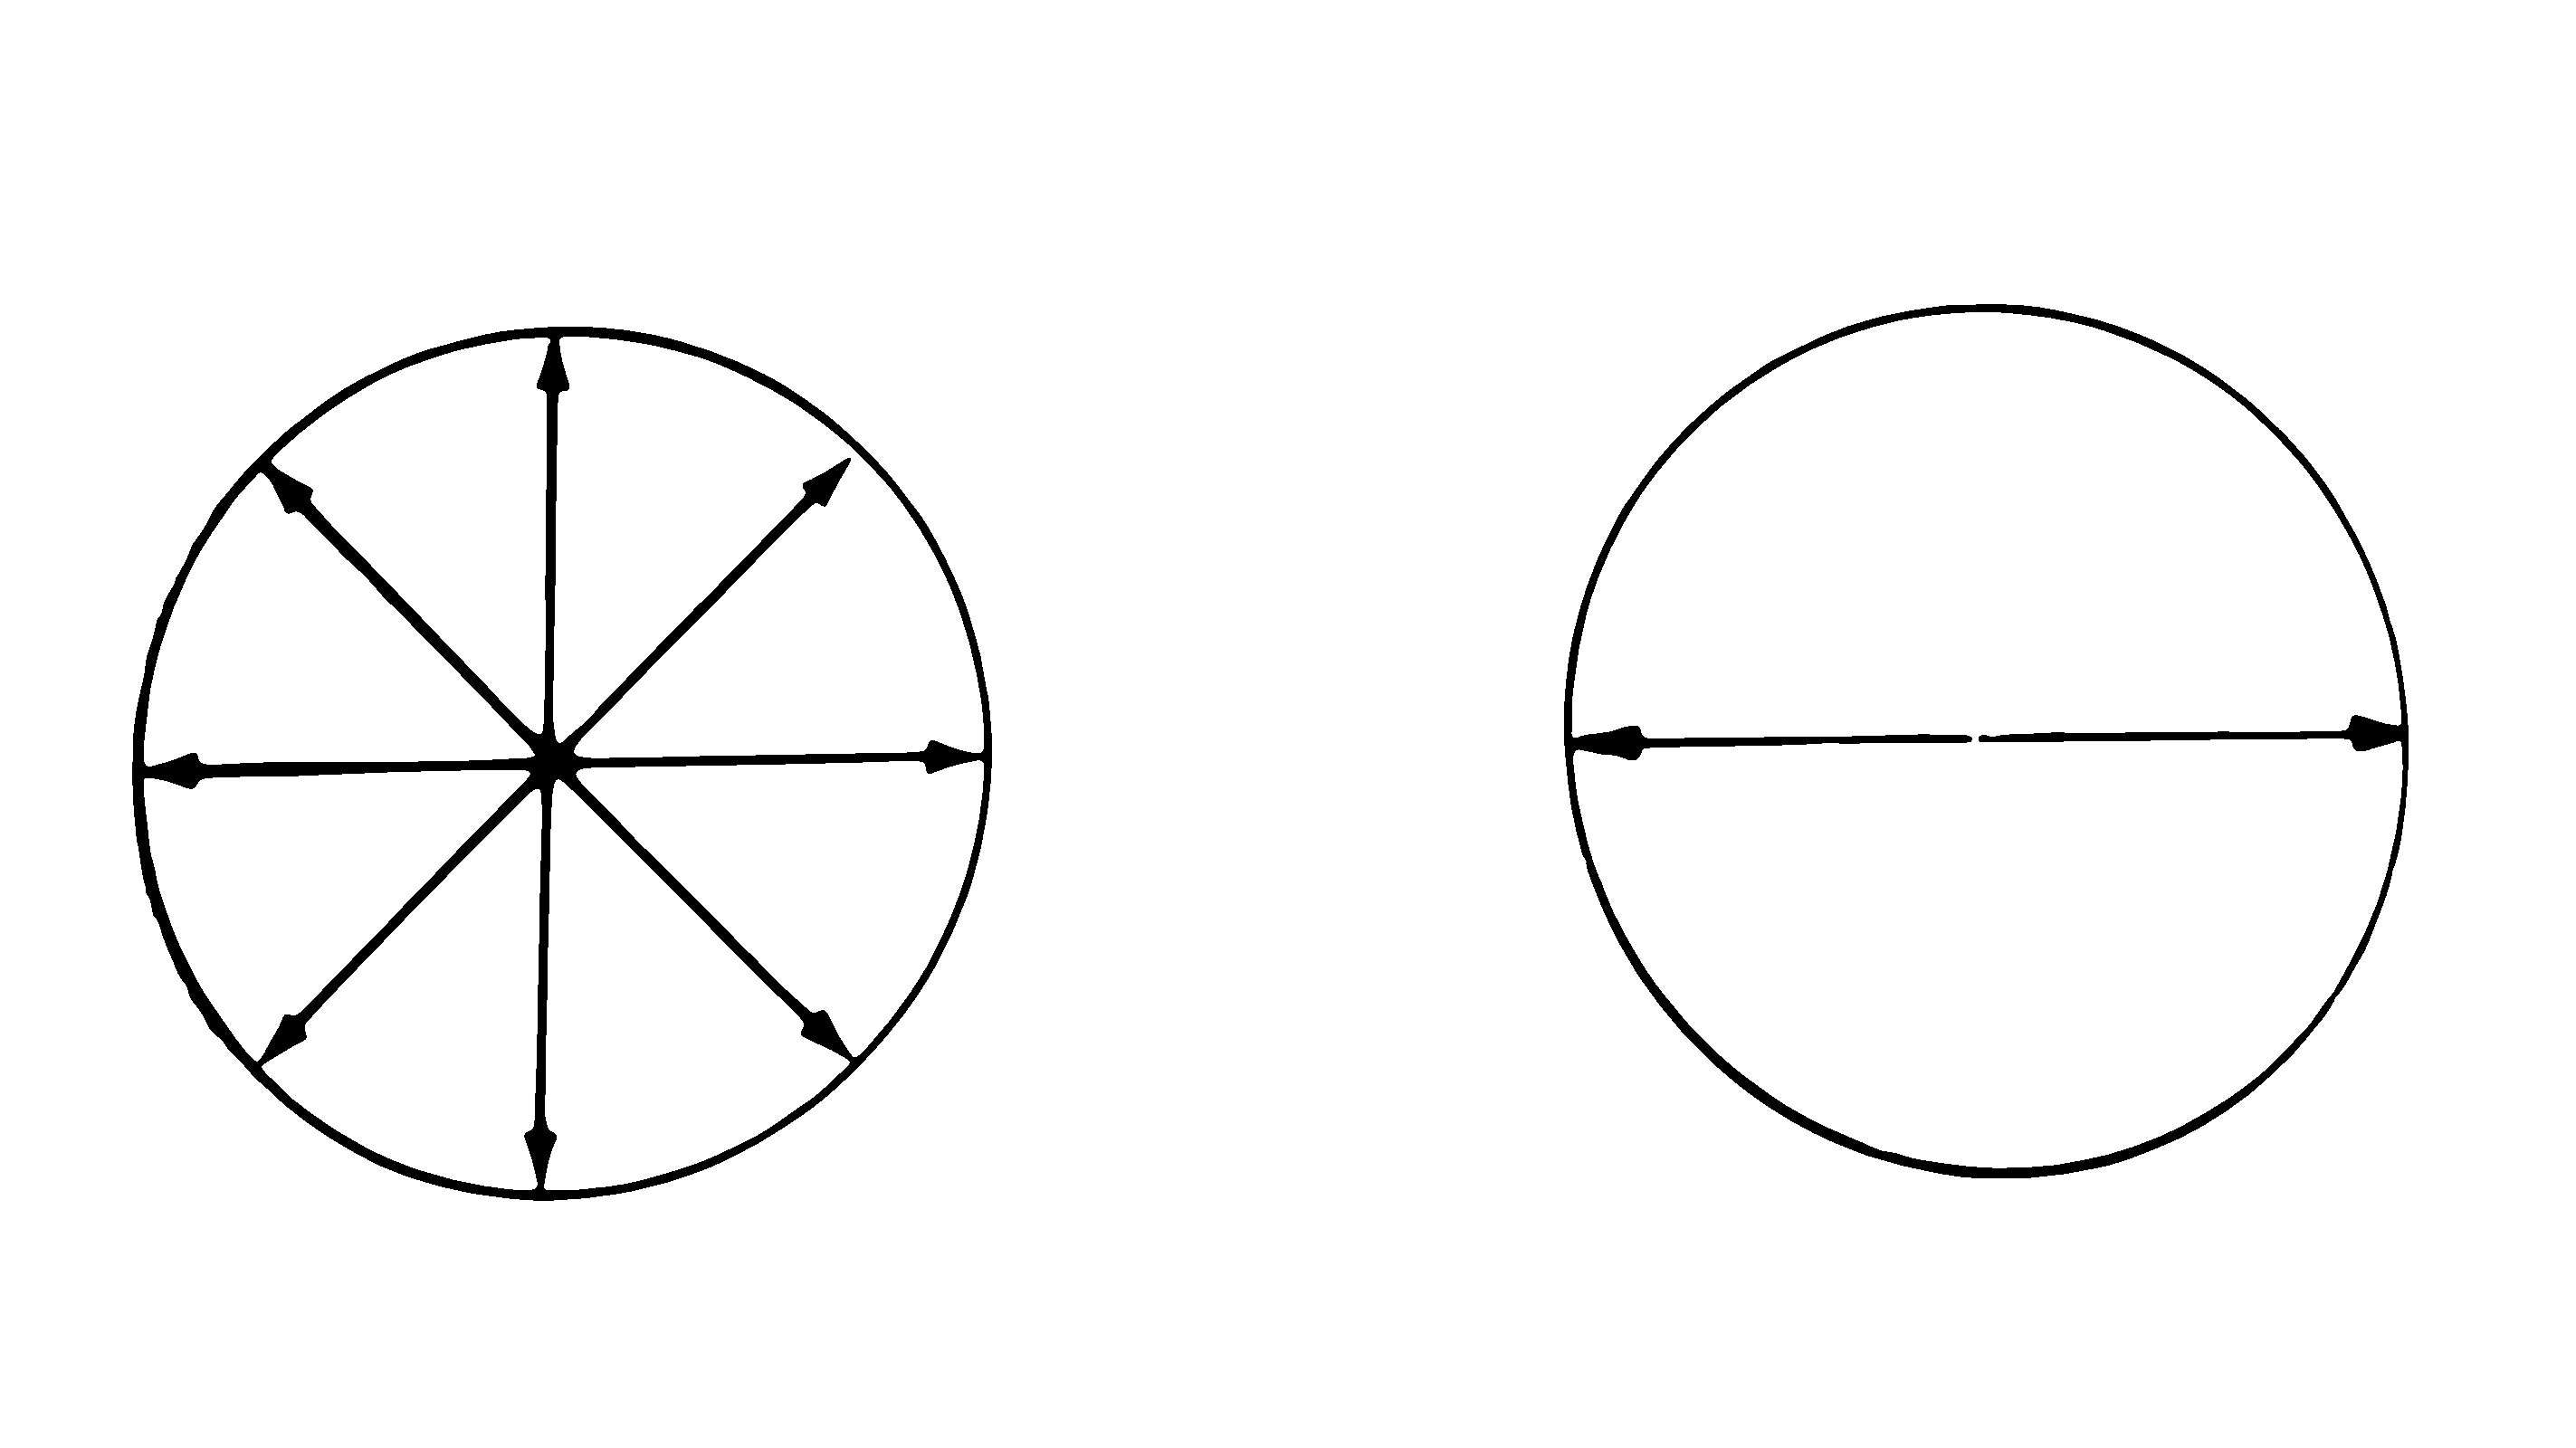
\includegraphics[width=0.5\textwidth,angle=0]{content/images/Figura_6_1.pdf}
    \caption{Vetores elétricos de um feixe de lux comum (esquerda) e polarizada (direita).}
    \label{figura_6_1}
\end{figure}

A luz polarizada (ou, mais propriamente, plano-polarizada) é aquela em que um dos vetores componentes foi removido. A vibração electromagnética resultante está, portanto, em um plano bem definido. Existem inúmeros modos de se conseguir este tipo de polarização um dos quais se utiliza do \textit{prisma de Nicol}. Esse tipo de prisma divide a luz ordinária incidente em dois feixes polarizados em planos perpendiculares.

A Figura \ref{figura_6_2} mostra, esquematicamente, um polarímetro. A luz monocromática ordinária (usualmente luz monocromática de sódio) entra através de um prisma (o polarizador) e é convertida em luz plano-polarizada que atravessa a célula de amostra e chega a outro prisma de Nicol, o chamado \textit{analisador}. Se não há amostra no tubo, a luz polarizada guarda seu aparelho e sua orientação fixa o plano que serve de origem aos ângulos. O prisma analisador pode ser girado à vontade e quando atinge a orientação adequada, toda a luz que a ele chega é capaz de atravessá-lo. A noventa graus dessa orientação a luz não pode atravessá-lo por não estar vibrando neste plano e o campo do visor fica escuro. Para rotações entre estas duas situações a luz é parcialmente transmitida. Os ângulos correspondentes podem ser lidos em um dispositivo semelhante a um transferidor.

\begin{figure}
    \centering
    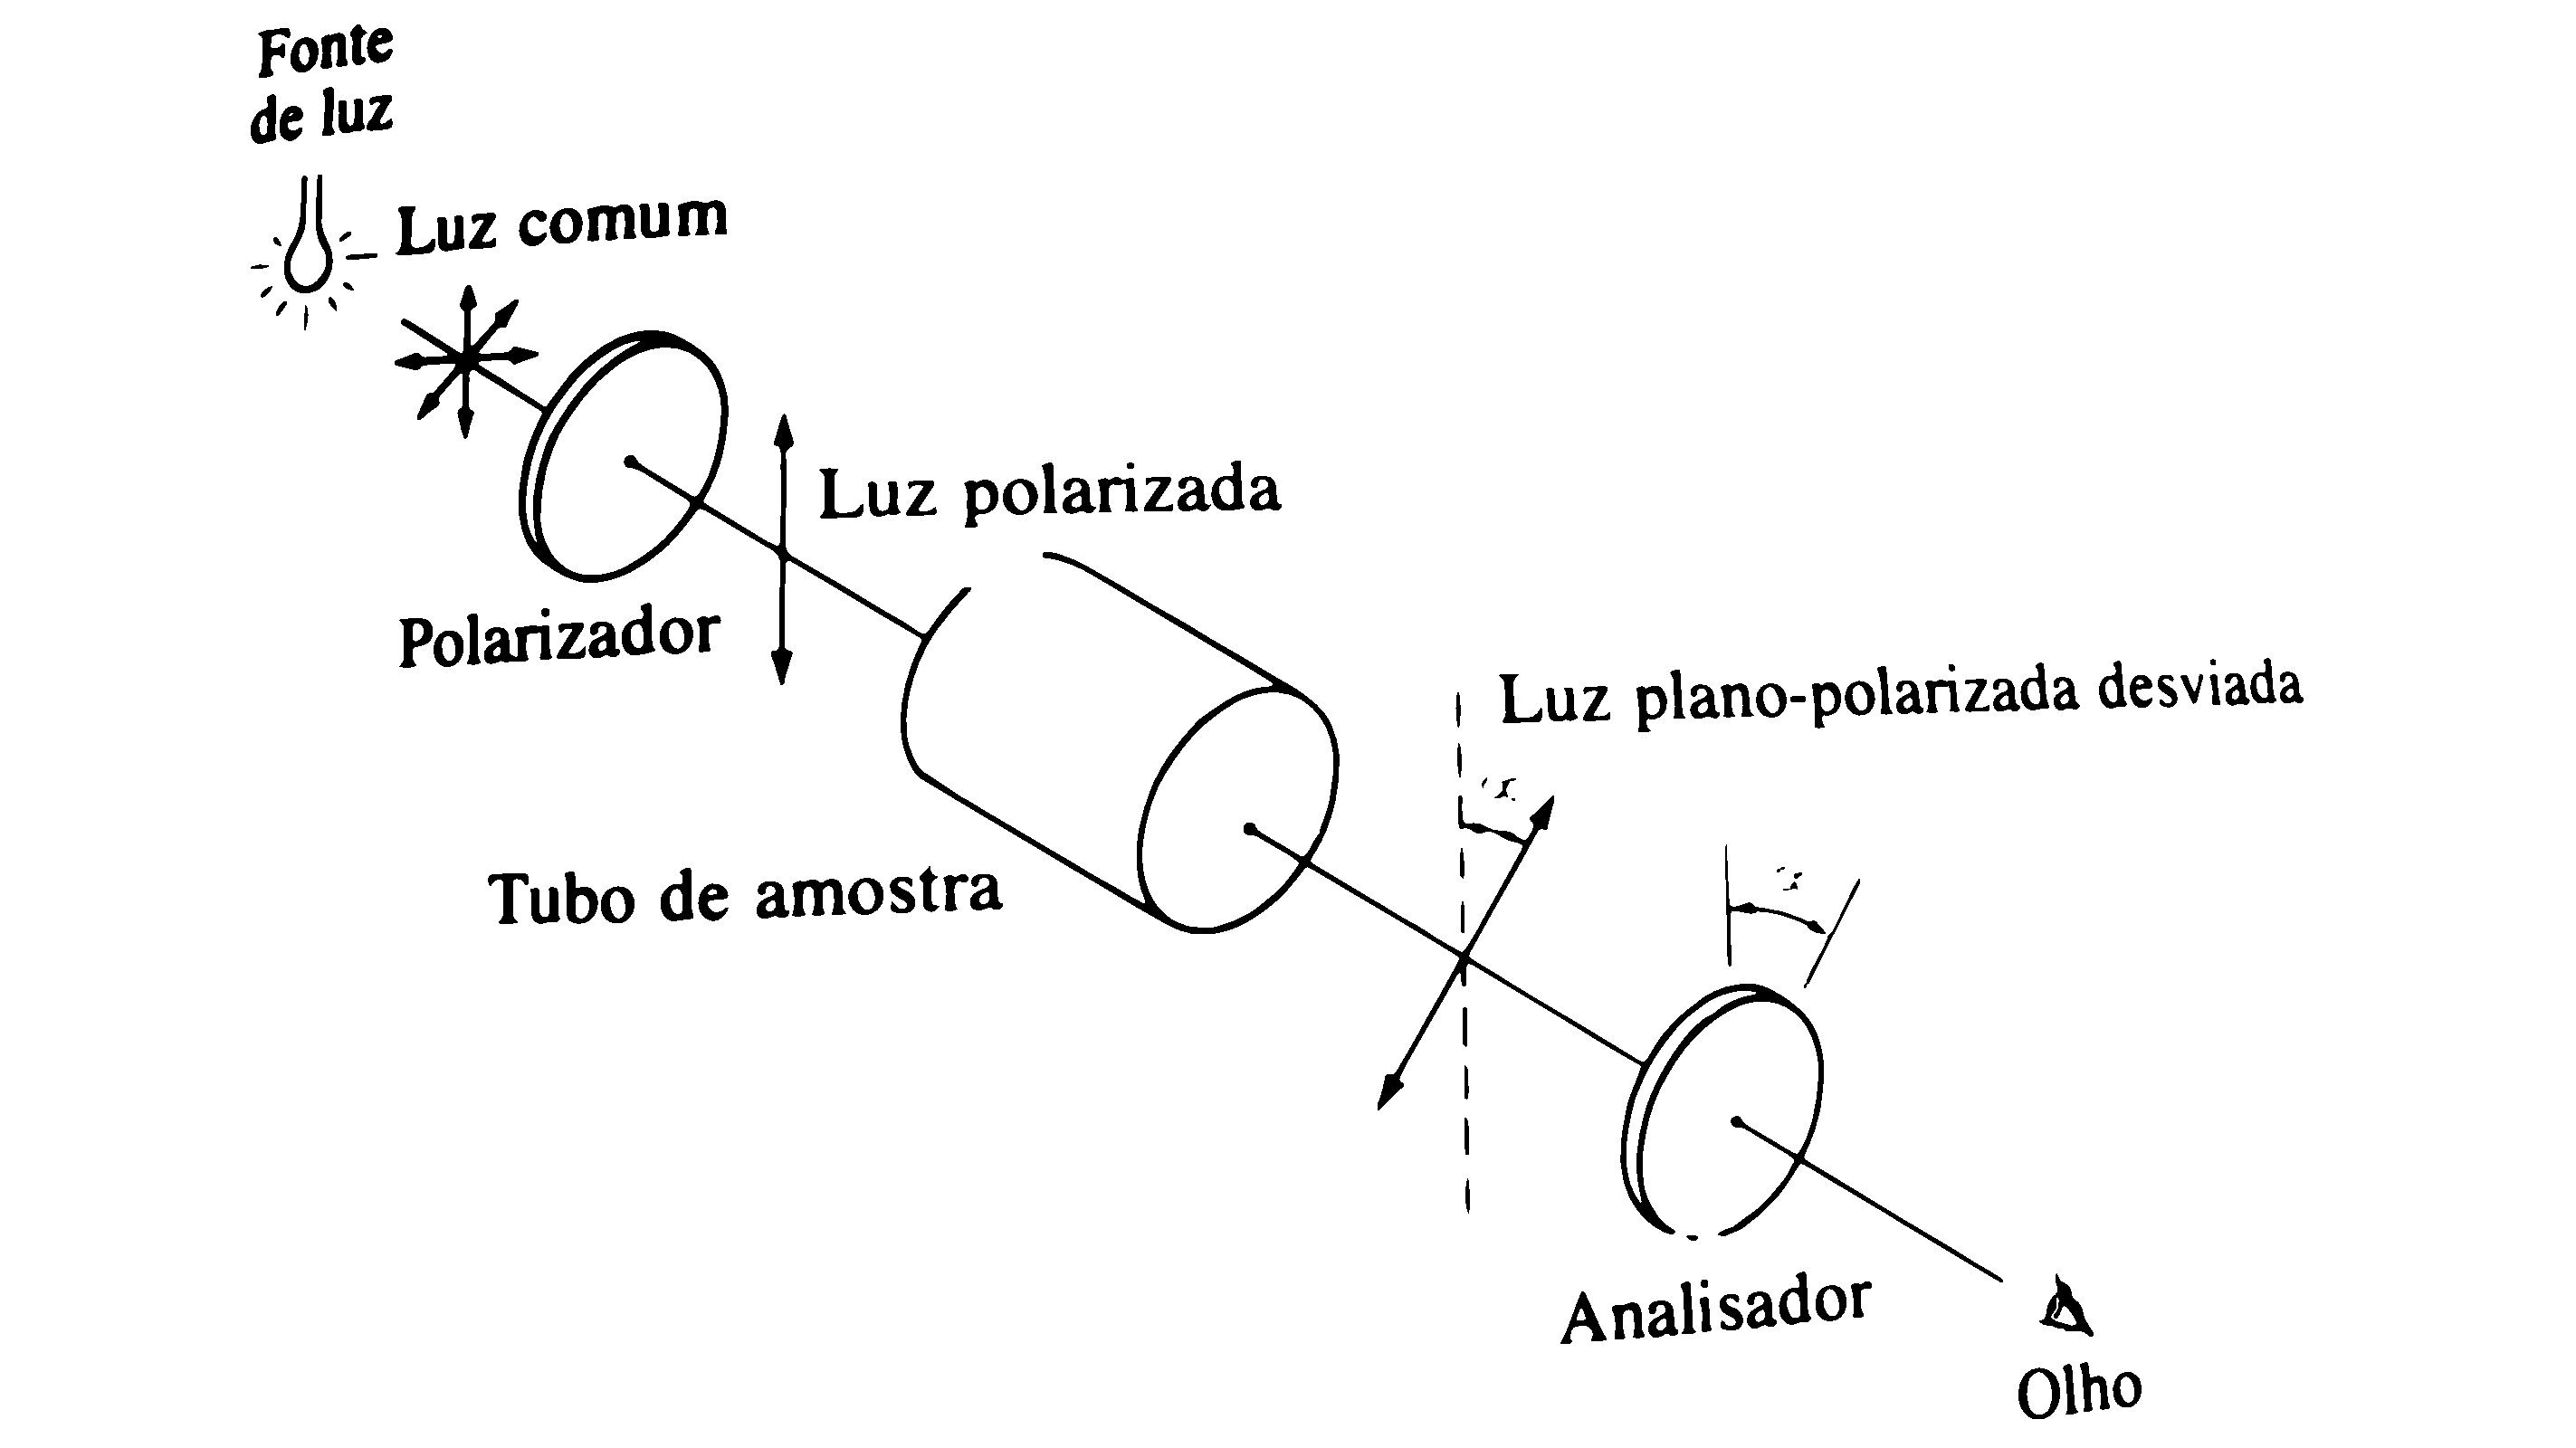
\includegraphics[width=0.7\textwidth,angle=0]{content/images/Figura_6_2.pdf}
    \caption{Representação esquemática de um polarímetro.}
    \label{figura_6_2}
\end{figure}

Quando o tubo de amostra está vazio, o máximo de luz transmitida ocorre para um angulo de rotação do analisador do 0$\degree$. Se substâncias comuns, como a água ou solução salina, são colocadas no tubo de amostra, o máximo de transmissão ainda coincide com a rotação de 0$\degree$ do analisado. Para certas outras substâncias, contudo, ocorre diferentemente. Por exemplo, para uma solução de açúcar,  o analisador tem de sair da posição de 0$\degree$, para que se possa observar um máximo na transmitância. O valor dessa rotação depende da concentração da solução, do comprimento do tubo de amostra, da temperatura, do comprimento de onda da luz utilizada e do solvente.

Para comparar com precisão as medidas de polarizada ode varias amostras, todas as variáveis têm de ser especificadas. Para converter as medidas a uma base mais sistemática, define-se uma quantidade chamada \textit{rotação especifica}, [$\alpha$]. como sendo a rotação em graus produzida em luz plano-polarizada por 1 g de substância em 1 mL de solução quando o comprimento da célula é de 1 decímetro. O valor da rotação, que pode ser direta (sentido dos ponteiros do relógio, positiva) ou inversa (sentido oposto, negativa), é, então, uma característica do composto examinado, desde que as demais variáveis sejam mantidas constantes.

\begin{equation}
    [\alpha] = \dfrac{\text{rotação observada}}{\text{comprimento do tubo (dm)} \times \text{concentração (g$\cdot$mL$^{-1}$)}}
\end{equation}

\noindent A linha $D$ do sódio (a linha de 5893 \AA, que dá a cor amarela à chama do sódio) é a fonte luminosa mais frequentemente usada e a temperatura mais comum é 25$\degree$C. A notação $[\alpha]_D$ fornece essas informações. Uma vez que a rotação especifica depende do solvente e da concentração (neste caso em gramas por 100 mL), é costume especificar a concentração e o solvente em seguida ao valor de $[\alpha]_D$. Por exemplo:

\begin{equation}
    [\alpha]_D = -32.3 \degree \enspace \text{\ch{CHCl3}} \enspace (c \enspace 2.05)
\end{equation}

\section{ENANTIÔMEROS E MISTURAS RACÊMICAS}

A interpretação correta do fenômeno da atividade ótica foi feita independentemente, por van't Hoff, na Holanda, e Le Bel, em Paris, em 1874. Os fatos experimentais exigem que se postule a geometria de um tetraedro regular para o átomo de carbono. Esta geometria, por outro lado, explica plenamente os fatos experimentais. Antes dessa época os químicos consideravam impossível saber qualquer coisa a respeito do arranjo especial das estruturas das moléculas - por arranjo espacial da estrutura entendemos a ordem em que os átomos se combinam para formá-la.

As propriedades geométricas do tetraedro são tais que, se houver quatro substituintes \textit{diferentes} ligados ao átomo de carbono, a molecular não conterá nenhum plano de simetria e isto acarreta a existência de dois arranjos geométricos diferentes para os quatro grupos ligados ao carbono. A diferença entre estes dois arranjos (\textit{configurações}) é que as duas estruturas não são superponíveis, átomo por átomo. Na verdade, as duas estruturas são \textit{imagens especulares não superponíveis} uma da outra (Figura \ref{figura_6_3}).

% \begin{figure}[H]
%     \centering
%     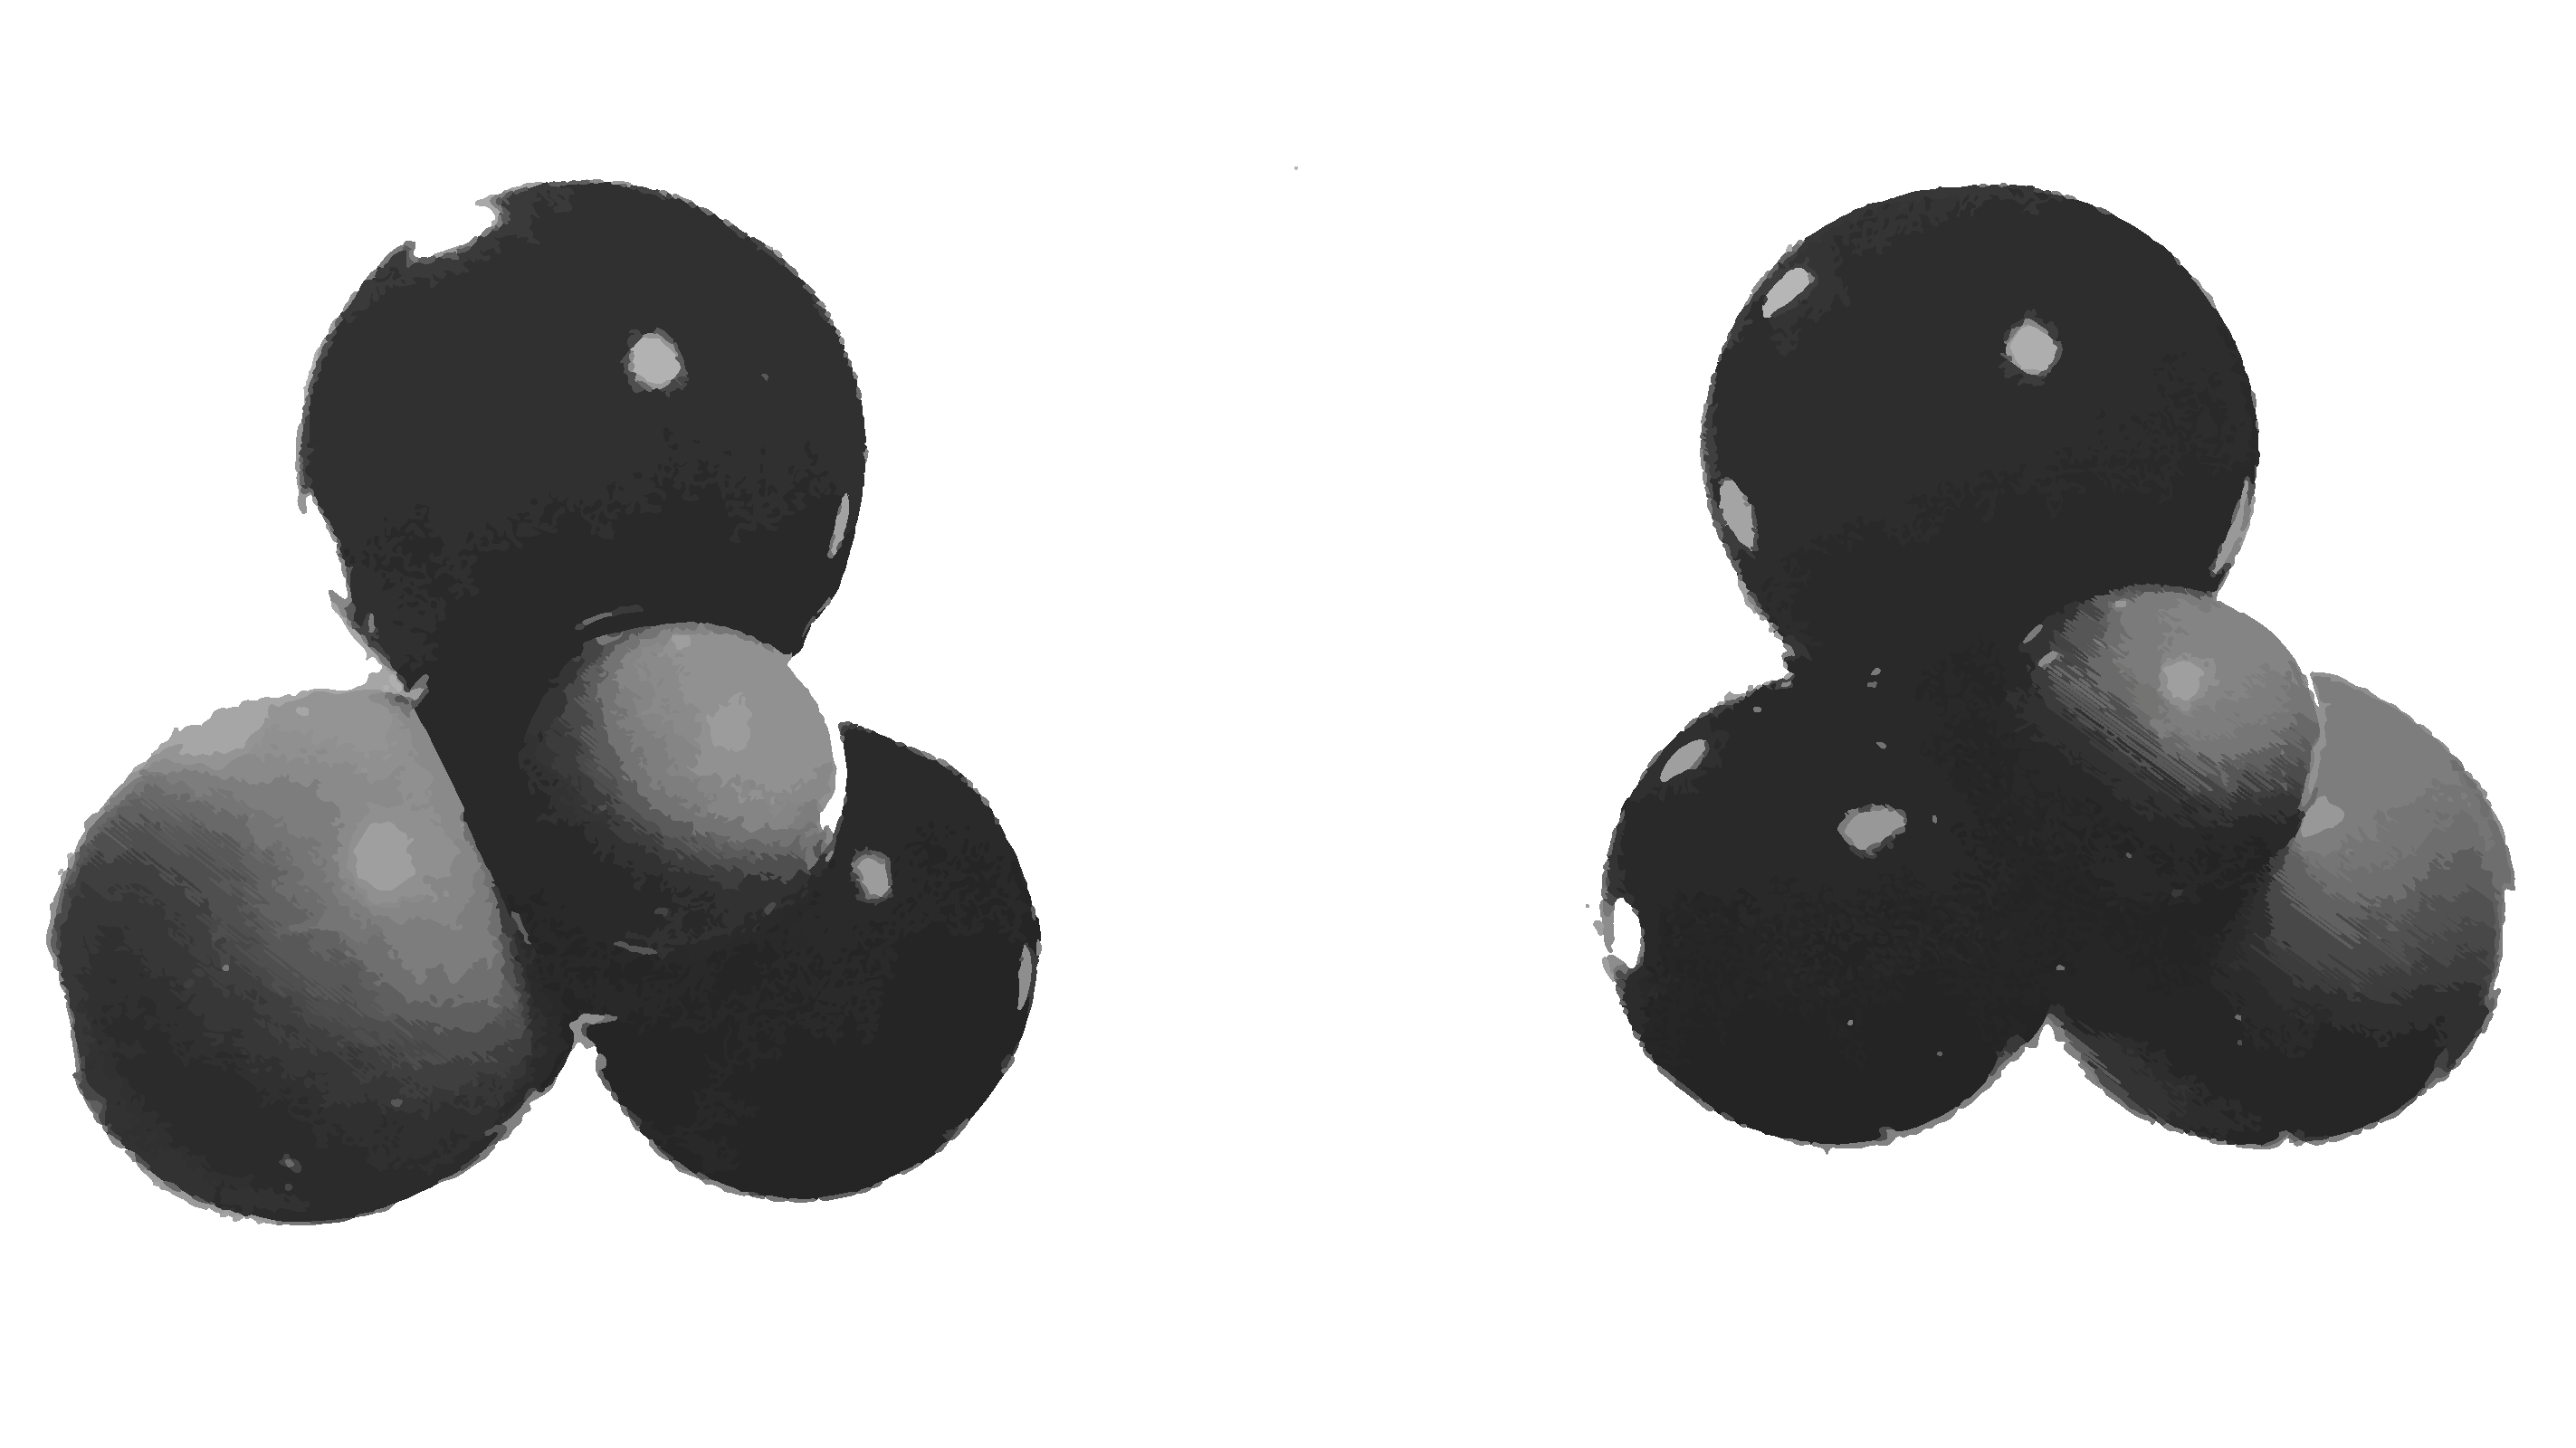
\includegraphics[width=0.5\textwidth,angle=0]{content/images/Figura_6_3.pdf}
%     \caption{Imagens especulares não superponíveis.}
%     \label{figura_6_3}
% \end{figure}

\begin{figure}[H]
    \centering
    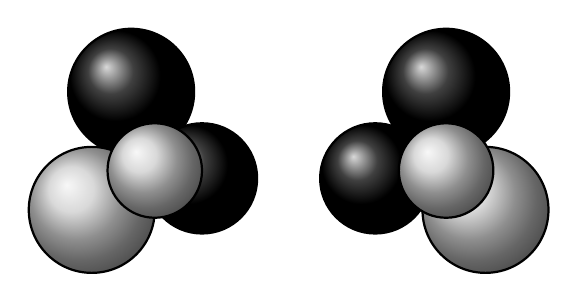
\begin{tikzpicture}[help lines/.style={thin,draw=black!50}] 
        %\draw[help lines] (0,0) grid (12,4);
        \shade[ball color = black] (2,3) circle (0.8cm);
        \draw[thick] (2,3) circle (0.8cm);
        \shade[ball color = black] (2.9,1.9) circle (0.7cm);
        \draw[thick] (2.9,1.9) circle (0.7cm);
        \shade[ball color = gray!40] (1.5,1.5) circle (0.8cm);
        \draw[thick] (1.5,1.5) circle (0.8cm);
        \shade[ball color = gray!40] (2.3,2) circle (0.6cm);
        \draw[thick] (2.3,2) circle (0.6cm);
        \begin{scope}[xscale=-1,xshift=-8cm]
            \shade[ball color = black] (2,3) circle (0.8cm);
            \draw[thick] (2,3) circle (0.8cm);
            \shade[ball color = black] (2.9,1.9) circle (0.7cm);
            \draw[thick] (2.9,1.9) circle (0.7cm);
            \shade[ball color = gray!40] (1.5,1.5) circle (0.8cm);
            \draw[thick] (1.5,1.5) circle (0.8cm);
            \shade[ball color = gray!40] (2.0,2) circle (0.6cm);
            \draw[thick] (2.0,2) circle (0.6cm);
        \end{scope}
    \end{tikzpicture}
    \caption{Imagens especulares não superponíveis.}
    \label{figura_6_3}
\end{figure}

\noindent Tais moléculas resultam da ligação de quatro grupos diferentes ao carbono e são chamadas de \textit{assimétricas} ou, então, de moléculas que contêm um \textit{carbono assimétrico}.

\begin{figure}[H]
    \centering
    \chemfig[][scale=0.7]{[1]d>(-[2]a)(<[7]c)(<:[6]b)}
    \qquad\qquad
    \chemfig[][scale=0.7]{[1]c>(-[2]a)(<[7]d)(<:[6]b)}
\end{figure}

\noindent\emph{No decorrer do texto adotaremos a seguinte convenção. A ligação que está no plano do papel é indicada por um traço fino, as que estão para a frente do plano são indicadas por uma cunha em negrito: finalmente, as que estão para trás são indicadas por uma cunha tracejada. Reservaremos o uso de uma linha fina tracejada para indicar outras ideias, como, por exemplo, que uma ligação está parcialmente rompida.}

Se dois compostos são imagem especular não superponível um do outro são chamados de \textit{enanciômeros}. Encontra-se experimentalmente que os enanciômeros possuem propriedades físicas idênticas., como era de se esperar, exceto a de rotação da luz polarizada, que é feita em direções opostas (e pelo mesmo ângulo). O 2-cloro-butano é um exemplo desta situação, já que existe como um par de enanciômeros.

\begin{figure}[H]
    \centering
    \begin{tikzpicture}[help lines/.style={thin,draw=black!50}] 
        %\draw[help lines] (0,0) grid (4,4);
        \draw[dashed,thick] (2,1) node[yshift=-2ex] {\footnotesize{Imagens especulares não superponíveis}} -- (2,3) node[yshift=2ex] {\footnotesize{Plano do espelho}};
        \node at (0,2) {\chemfig[][scale=0.7]{C_2H_5>C(<:[1]H)(<:[7]Cl)(<CH_3)}};
        \node at (4,2) {\chemfig[][scale=0.7]{CH_3>C(<:[1]H)(<:[7]Cl)(<C_2H_5)}};
    \end{tikzpicture}
\end{figure}

\noindent O leitor deveria construir modelos destes enanciômeros e convencer-se de que eles não são superponíveis.

Se dois enanciômeros são misturados em quantidades iguais, o resultado é o que chamamos de \textit{mistura racêmica}, que não muda o plano da luz polarizada porque o desvio de cada enanciômeros cancela o do outro. 

Cotidianamente deparamos com uma série de enanciômeros. Por exemplo, a mão esquerda é a imagem especular da mão direita, e as duas mãos, como bem o sabemos, não se superpõem. Isso fica obvio quando tentamos vestir uma luva de mão direita na mão esquerda. Da mesma forma, nossos sapatos guardam entre si uma relação enanciomérica e o estoque de uma sapataria exemplifica uma mistura racêmica.

Se a molécula é superponível à sua imagem especular (molécula e imagem são idênticas), tal substância não pode existir como um par de enanciômeros, e sim como um composto que não desvia o plano da luz polarizada. Com moléculas simples, é fácil determinar se a atividade ótica será observada ou não. Se dois ou mais átomos ou grupos de átomos ligados ao carbono são iguais, então não haverá carbono assimétrico, as imagens especulares serão superponíveis e as estruturas correspondentes serão idênticas, isto é, a mesma molécula. O 2-cloro-propano exemplifica isto.

\begin{figure}[H]
    \centering
    \begin{tikzpicture}[help lines/.style={thin,draw=black!50}] 
        %\draw[help lines] (0,0) grid (4,4);
        \draw[dashed,thick] (2,1) node[yshift=-2ex] {\footnotesize{Imagens especulares superponíveis}} -- (2,3) node[yshift=2ex] {\footnotesize{Plano do espelho}};
        \node at (0,2) {\chemfig[][scale=0.7]{CH_3>C(<:[1]H)(<:[7]Cl)(<CH_3)}};
        \node at (4,2) {\chemfig[][scale=0.7]{CH_3>C(<:[1]H)(<:[7]Cl)(<CH_3)}};
    \end{tikzpicture}
\end{figure}

\noindent Comparemos esse composto com o 2-cloro-butano em que todos os grupos ligados ao carbono 2 são diferentes. Em compostos simples, a presença de um átomo de carbono assimétrico levará à existência de enanciômeros.

Vale a pena perguntar se os isômeros óticos não passam de curiosidade acadêmica ou se eles têm importância no nosso mundo real. Como ficará claro em capítulos posteriores, muitos, e na, verdade a maioria, dos compostos que ocorrem em sistemas vivos contêm um ou mais átomos de carbono assimétrico. Os sistemas biológicos são particularmente exigentes em relação aos isômeros óticos que preferem e é de suma importância compreender este fenômeno se quisermos compreender os sistemas vivos.

\noindent\emph{Também podemos perguntar: Por que os enanciômeros comportam-se desta maneira em relação à luz polarizada? Se examinarmos uma solução de um composto, um líquido ou gás puros, por exemplo metano, verificamos que eles contêm moléculas orientadas de todos os modos possíveis. Uma dada molécula em uma orientação arbitrariamente fixada desviara o plano de polarização de luz de um pequeno ângulo, digamos, para a esquerda. Se a molécula é superponível à sua imagem especular, como é o caso do metano, é igualmente provável que a luz venha encontrar outra molecular com uma orientação correspondente à imagem especular da primeira em um dado instante do percurso. As contribuições rotacionais das duas moléculas serão, então, iguais, opostas e se cancelarão. Ao trabalharmos com uma amostra macroscópica as varias orientações possíveis desviarão o plano de rotação da luz com diferentes intensidades e em diferentes direções, mas as compensações farão com que a rotação total seja sempre zero na média.}

\emph{Se dispusermos, por outro lado, de uma solução composta de moléculas idênticas, porém não superponíveis a suas imagens especulares, correspondendo a um mesmo enanciômero, cada molécula poderá estar em diferentes orientações de modo que cada uma contribuirá para a rotação ótica da solução como um todo. Mas como a imagem especular de cada orientação corresponde ao enanciômero que não está presente, as rotações não se cancelam, somando-se para dar como resultado um valor qualquer diferente de zero. O outro enanciômero em solução teria um comportamento correspondente e, portanto, um desvio de igual angulo em sentido oposto. Uma mistura constituída de quantidades iguais orientação, haveria uma probabilidade igual de ocorrência de sua imagem especular e a rotação resultante de tal mistura seria zero.}

\section{PROJEÇÕES DE FISCHER}

É difícil fazer a representação tridimensional de um tetraedro com um desenho ou uma formula a duas dimensões. As duas representações adequadas são as \textit{formulas em perspectiva} (Seção 3.1) e de \textit{projeção}. No presente texto usaremos ambas. As formulas de projeção mostram apenas duas dimensões, sendo a terceira perpendicular ao pano do papel. As \textit{projeções de Fischer} são bastante usadas por causa de sua simplicidade (Figura \ref{figura_6_4}).

\begin{figure}[H]
    \centering
    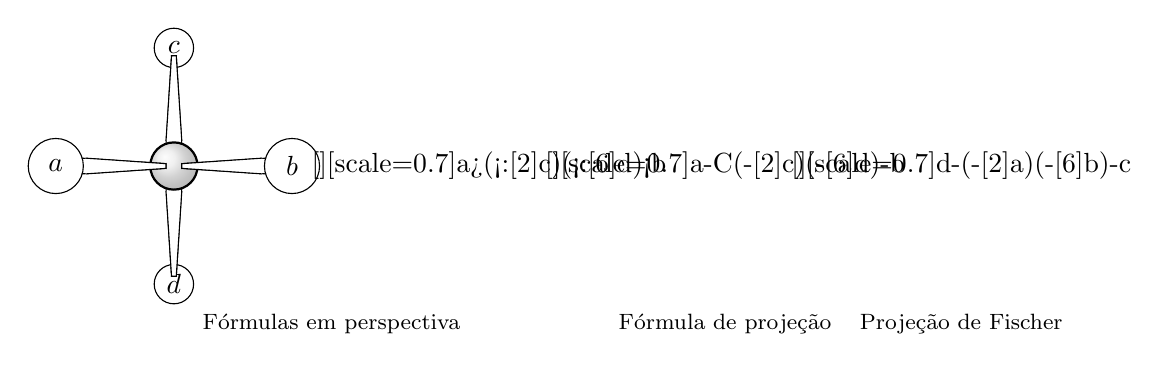
\begin{tikzpicture}[help lines/.style={thin,draw=black!50}] 
       % \draw[help lines] (0,0) grid (12,4);
        \shade[ball color = gray!40, opacity = 0.4] (2,2) circle (0.3cm);
        \draw[thick] (2,2) circle (0.3cm);
        \draw (3.5,2) circle (0.35cm) node {$b$};
        \draw (0.5,2) circle (0.35cm) node {$a$};
        \draw (2,3.5) circle (0.25cm) node {$c$};
        \draw (2,0.5) circle (0.25cm) node {$d$};
        \draw[rounded corners=1pt] (2.1,1.72) -- (2.03,0.6) -- (1.97,0.6) -- (1.9,1.72);
        \draw[rounded corners=1pt] (2.1,2.28) -- (2.03,3.4) -- (1.97,3.4) -- (1.9,2.28);
        \path[draw,fill=white] (2.1,1.68) -- (2.03,0.6) -- (1.97,0.6) -- (1.9,1.68);
        \path[draw,fill=white] (2.1,2.32) -- (2.03,3.4) -- (1.97,3.4) -- (1.9,2.32);
        \draw[rounded corners=1pt] (0.83,2.1) -- (1.90,2.03) -- (1.90,1.97) -- (0.83,1.9);
        \draw[rounded corners=1pt] (3.17,2.1) -- (2.10,2.03) -- (2.10,1.97) -- (3.17,1.9);
        \path[draw,fill=white] (0.88,2.1) -- (1.90,2.03) -- (1.90,1.97) -- (0.88,1.9);
        \path[draw,fill=white] (3.12,2.1) -- (2.10,2.03) -- (2.10,1.97) -- (3.12,1.9);
        \node at (6,2) {\chemfig[][scale=0.7]{a>(<:[2]c)(<:[6]d)<b}};
        \node at (4,0) {\footnotesize{Fórmulas em perspectiva}};
        \node at (9,2) {\chemfig[][scale=0.7]{a-C(-[2]c)(-[6]d)-b}};
        \node at (9,0) {\footnotesize{Fórmula de projeção}};
        \node at (12,2) {\chemfig[][scale=0.7]{d-(-[2]a)(-[6]b)-c}};
        \node at (12,0) {\footnotesize{Projeção de Fischer}};
    \end{tikzpicture}
    \caption{Quatro representações equivalentes de um carbono tetraédrico.}
    \label{figura_6_4}
\end{figure}

Por convenção, as linhas horizontais são imaginadas para cima do plano da página, enquanto que as verticais são entendidas como ligações que se dirigem para baixo do papel. Manipulemos agora algumas destas fórmulas para mostrar claramente o que representam.

\begin{figure}[H]
    \centering
    \schemestart
        \chemfig[][scale=0.7]{a-(-[2]c)(-[6]d)-b}
        \qquad\text{\footnotesize{e}}\qquad
        \chemfig[][scale=0.7]{b-(-[2]d)(-[6]c)-a}
    \schemestop
\end{figure}

\noindent Em uma projeção de Fischer, as duas formulas referem-se à mesma molécula. É fácil vermos porque, desenhando as duas fórmulas em perspectiva correspondentes:

\begin{figure}[H]
    \centering
    \schemestart
        \chemfig[][scale=0.7]{a>(<:[2]c)(<:[6]d)<b}
        \qquad\text{\footnotesize{e}}\qquad
        \chemfig[][scale=0.7]{b>(<:[2]d)(<:[6]c)<a}
    \schemestop
\end{figure}

\noindent Se tomarmos a segunda fórmula e a rodarmos de 180$\degree$ no sentido direto, mantendo-a no plano da página.

\begin{figure}[H]
    \centering
    \schemestart
        \chemfig[][scale=0.7]{@{a2}b>(<:[2]d)(<:[6]c)<a@{a1}}
        \arrow{->}
        \chemfig[][scale=0.7]{a>(<:[2]c)(<:[6]d)<b}
    \schemestop
    \chemmove{\draw(a1).. controls +(south:1.2cm) and +(south:1.2cm).. (a2);}
\end{figure}

\noindent veremos que $a$ e $b$ mudaram de lugar, assim como $c$ e $d$, e que $a$ e $b$ ainda se projetam em nossa direção e $c$ e $d$ para trás do papel. Note que o que conseguimos com esta operação foi colocar a estrutura em uma situação idêntica à da primeira. A conclusão é que as duas fórmulas em perspectiva representam, neste caso, o mesmo composto. 

Vales a pena lembrar que a rotação de 180$\degree$ imposta a uma projeção de Fischer leva sempre à outra projeção, a qual corresponde a uma molécula idêntica. Por outro lado, as duas projeções de Fischer que se seguem não são idênticas e representam um par de enanciômeros:

\begin{figure}[H]
    \centering
    \schemestart
        \chemfig[][scale=0.7]{a-(-[2]c)(-[6]d)-b}
        \qquad\text{\footnotesize{e}}\qquad
        \chemfig[][scale=0.7]{d-(-[2]a)(-[6]b)-c}
    \schemestop
\end{figure}

\noindent Para demonstrar essa afirmativa escrevemos outra vez as fórmulas em perspectiva correspondentes:

\begin{figure}[H]
    \centering
    \schemestart
        \chemfig[][scale=0.7]{a>(<:[2]c)(<:[6]d)<b}
        \qquad\text{\footnotesize{e}}\qquad
        \chemfig[][scale=0.7]{d>(<:[2]a)(<:[6]b)<c}
    \schemestop
\end{figure}

\noindent Para tentar superpô-las, tomamos a segunda estrutura e rodamos 90$\degree$ no sentido inverso, realizando a rotação no plano da página:

\begin{figure}[H]
    \centering
    \schemestart
        \chemfig[][scale=0.7]{d>(<:[2]a@{a2})(<:[6]b)<c@{a1}}
        \arrow{->}
        \chemfig[][scale=0.7]{a>:(<[2]c)(<[6]d)<:b}
    \schemestop
    \chemmove{\draw(a1).. controls +(90:0.5cm) and +(45:0.5cm).. (a2);}
\end{figure}

Se compararmos agora a estrutura obtida com a premeria, podemos ver que os grupos estão ligados ao carbono assimétrico na mesma ordem, em outras palavras, começando com o grupo $a$, no sentido direto a ordem é $acbd$, em ambas as estruturas. Porém os grupos que vice-versa. Isto significa que as duas estruturas aparecem acima do plano na outra estrutura e sendo o plano do papel o plano do espelho. Portanto, as fórmulas de projeção que escrevemos representam um par de enanciômero e têm configurações opostas em torno do átomo de carbono assimétrico. 

O método acima pode ser sempre usado para se descobrir se duas projeções de Fischer correspondem à mesma molécula ou a enanciômeros. Entretanto, essa verificação é bastante laboriosa e leva facilmente a erro. Para simplificar a questão os químicos desenvolveram uma regra simples: para um composto que contém apenas um carbono assimétrico \textit{a troca de dois grupos quaisquer na projeção de Fischer converte a molécula no seu enanciômero}. Considere o exemplo abaixo:

\begin{figure}[H]
    \centering
    \schemestart
        \chemfig[][scale=0.7]{a-(-[2]c)(-[6]d)-b}
        \qquad\text{\footnotesize{trocando $a$ por $d$, obtém-se}}\qquad
        \chemfig[][scale=0.7]{d-(-[2]c)(-[6]a)-b}
    \schemestop
\end{figure}

\noindent que é o enanciômero da primeira molécula.

Suponhamos agora que nós tomamos a segunda fórmula e trocamos dois grupos. Isso nos leva ao enanciômero da segunda fórmula, isto é, nos leva de volta à primeira estrutura. Em outras palavras, o que fizemos foi trocar $a$ e $d$ mais uma vez. Podemos trocar, entretanto, \textit{quaisquer} dois grupos para obter um enanciômero. Usemos a segunda fórmula e troquemos dois outros grupos:

\begin{figure}[H]
    \centering
    \schemestart
        \chemfig[][scale=0.7]{d-(-[2]c)(-[6]a)-b}
        \qquad\text{\footnotesize{trocando $a$ por $c$, obtém-se}}\qquad
        \chemfig[][scale=0.7]{d-(-[2]a)(-[6]c)-b}
    \schemestop
\end{figure}

